\section{Benchmarks on parallel frameworks}\label{sec:parallel}

As aforementioned, FOODIE is unaware of any parallel paradigms or programming models the client codes adopt. As a consequence, the parallel performances measurements presented into this section are aimed only to prove that FOODIE environment does not destroy the parallel scaling of the baseline code implemented without FOODIE.

To obtain such a prove, the 1D Euler PDE system described previously is numerically solved with FOODIE-aware test codes that in turn exploit parallel resources by means:

\begin{itemize}
  \item CoArray Fortran (CAF) model, for shared and distributed memory architectures;
  \item OpenMP directive-based model, for only shared memory architectures;
  \item Message Passing Interface (MPI) library-based model, for only distributed memory architectures;
  \end{itemize}

In order to measure the performances of the parallel-enabled FOODIE tests, the \emph{strong} and \emph{weak} scaling have been considered. For the strong scaling the \emph{speedup} has been computed:

\begin{equation}
  speedup(N, k) = \frac{T_{serial}(N)}{T_{parallel}(N, k)}
  \label{eq:strong-scaling-speedup}
\end{equation}
where $N$ is the problem size, $K$ the number of parallel resources used (namely the physical cores), $T_{serial}$ is the CPU time of the serial code and $T_{parallel}$ the one of the parallel code. The ideal speedup is linear with slop equals to 1. The efficiency correlated to the strong scaling measurement is defined as:

\begin{equation}
  efficiency(N, k) = \frac{speedup(N, k)}{k}
  \label{eq:strong-scaling-efficiency}
\end{equation}
The maximum ideal efficiency is obviously the unity.

For the of weak scaling measurement the \emph{sizeup} has been computed:

\begin{equation}
  sizeup(N, k) = \frac{N_k}{N_1} \cdot \frac{T_{serial}(N_1)}{T_{parallel}(N_k, k)}
  \label{eq:weak-scaling-sizeup}
\end{equation}
where $N_1$ is the minimum size considered and $N_K$ is the size used for the test computed with $k$ parallel resources. If $N_K$ is scaled proportional to $N_1$, the ideal sizeup is again linear and if $N_k = k \cdot N_1$ the slope is again linear. The efficiency correlated to the weak scaling is defined as:

\begin{equation}
  efficiency(N, k) = \frac{sizeup(N, k)}{k}
  \label{eq:weak-scaling-efficiency}
\end{equation}
The maximum ideal efficiency is obviously the unity.

The same 1D Euler PDE problem is also solved by parallel-enabled codes that are not based on FOODIE: their solutions provide a reference for measuring the effect of FOODIE abstraction on the parallel scaling.

\subsection{CAF benchmark}\label{subsec:caf}

{\color{red} To be written.}

\subsection{OpenMP benchmark}\label{subsec:openmp}

This subsection reports the parallel scaling analysis of Euler 1D test programs (with and without FOODIE) being parallelized by means of OpenMP directives-based paradigm. This parallel model is based on the concept of \emph{threads}: an OpenMP enabled code start a single (master) threaded program and, at run-time, it is able to generate a team of (many) threads that work concurrently on the parallelized parts of the code, thus reducing the CPU time necessary for completing such parts. The parallelization is made by means of \emph{directives} explicitly inserted by the programmer: the communications between threads are automatically handled by the compiler (through the provided OpenMP library used as back-end). OpenMP parallel paradigm is not a standard feature of Fortran, rather it is an extension provided by the compiler vendors. This parallel paradigm constitutes an effective and easy approach for parallelizing legacy serial codes, however its usage is limited to shared memory architectures because all threads must have access to the same memory.

\begin{figure}[!ht]
  \centering
  \begin{subfigure}[b]{0.80\textwidth}
    \centering
    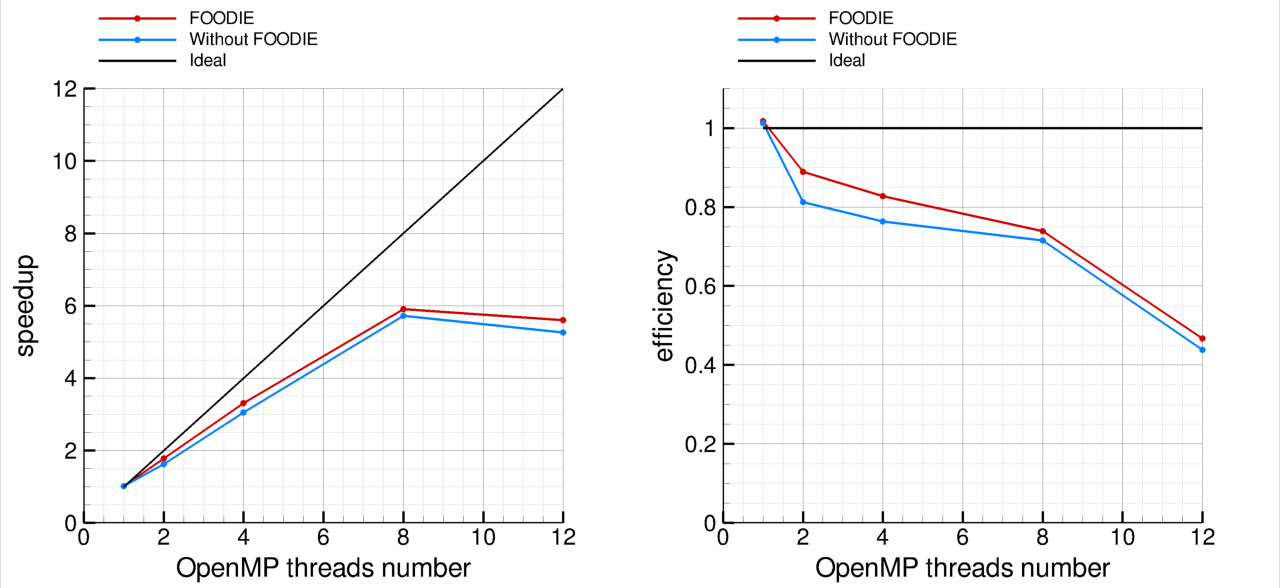
\includegraphics[width=1.00\textwidth]{openmp_benchmark/euler-1D-openmp/strong-scaling-comparison.png}
    \caption{Strong scaling, number of cells 240000}\label{fig:strong-scaling-openmp}
  \end{subfigure}\\
  \begin{subfigure}[b]{0.80\textwidth}
    \centering
    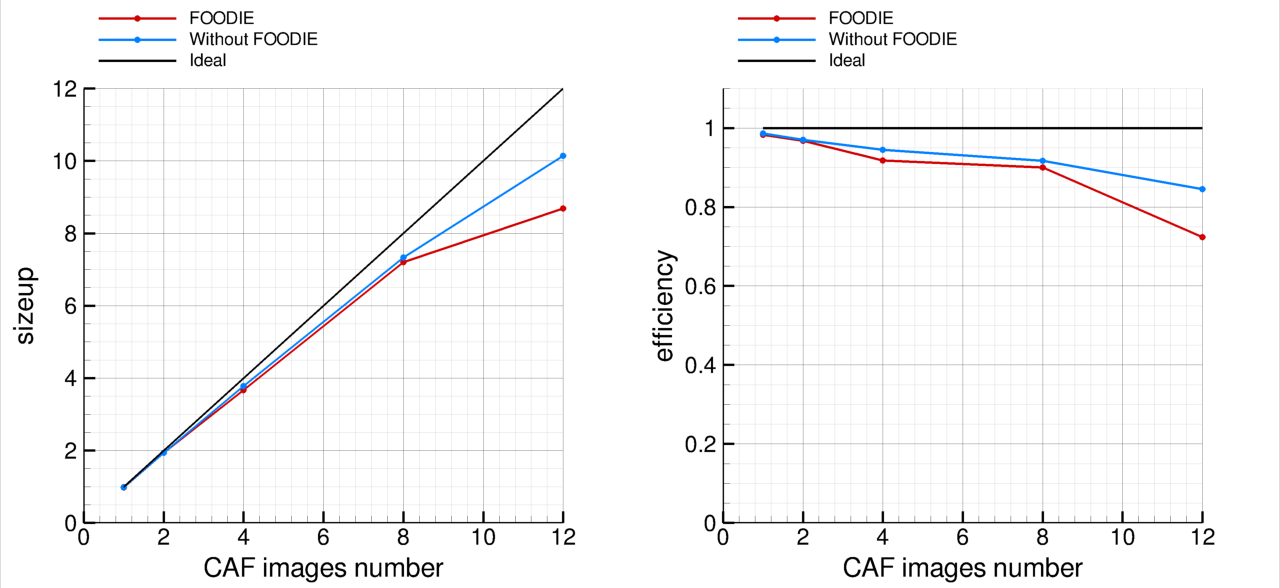
\includegraphics[width=1.00\textwidth]{openmp_benchmark/euler-1D-openmp/weak-scaling-comparison.png}
    \caption{Weak scaling, minimum number of cells 24000}\label{fig:weak-scaling-openmp}
  \end{subfigure}\\
  \caption{Scaling efficiency with OpenMP programming model}\label{fig:scaling-openmp}
\end{figure}

The benchmarks shown in this section have been done on a \emph{dual Intel(R) Xeon(R) CPU X5650} exacores workstation for a total of 12 physical cores, coupled with 24GB of RAM. In order to perform an accurate analysis 4 different codes have considered:

\begin{itemize}
  \item FOODIE-aware codes:
    \begin{itemize}
      \item serial code;
      \item OpenMP-enabled code;
      \end{itemize}
  \item procedural codes without using FOODIE library:
    \begin{itemize}
      \item serial code;
      \item OpenMP-enabled code;
      \end{itemize}
  \end{itemize}

These codes (see \ref{subsec:euler-1D-OpenMP-API} for the implementation details) have been compiled by means of the GNU gfortran compiler v5.2.0 with \emph{-O2 -fopenmp} compilation flags.

The Euler conservation laws are integrated for 30 time steps by means of the TVD RK(5,4) solver: the measured CPU time used for computing the scaling efficiencies is the average of the 30 integrations, thus representing the mean CPU time for computing one time step integration.

For the strong scaling, the benchmark has been conducted with 240000 finite volumes. Figure \ref{fig:strong-scaling-openmp} summarizes the strong scaling analysis: it shows that FOODIE-based code scales similarly to the baseline code without FOODIE.

For the weak scaling the minimum size is 24000 finite volumes and the size is scaled linearly with the OpenMP threads, thus $N_{12} = 288000$ cells. Figure \ref{fig:weak-scaling-openmp} summarizes the weak scaling analysis and it essentially confirms that FOODIE-based code scales similarly to the baseline code without FOODIE.

Both strong and weak scaling analysis point out that for the computing architecture considered the parallel scaling is reasonable up to 8 cores: using 12 cores the measured efficiencies become unsatisfactory, reducing below the 60\%.

To complete the comparison, the absolute CPU-time consumed by the two families of codes (with and without FOODIE) must be considered. Table \ref{tab:openmp-results} summarizes the benchmarks results. As shown, procedural and FOODIE-aware codes consume a very similar CPU-time for both the strong and the weak benchmarks. The same results are shown in figure \ref{fig:cpu-time-openmp}. These results prove that the abstraction of FOODIE environment does not degrade the computational efficiency.

\begin{table}[!ht]
  \centering
  \caption{OpenMP benchmarks results\label{tab:openmp-results}}
  \begin{subtable}[b]{0.80\textwidth}
    \centering
    \caption{Strong benchmarks, number of cells 240000\label{tab:openmp-results-strong}}
    \resizebox{1.00\textwidth}{!}{%
    \begin{tabular}{ccccc}
      {\sc Number of OpenMP threads} & \multicolumn{4}{c}{\sc CPU time for 1 time step integration}              \\
      \hline
                                     & FOODIE serial & FOODIE parallel & procedural serial & procedural parallel \\
      \cmidrule{2-5}
      1                              & 3.3466        & 3.3076          & 3.1252            & 3.0873              \\
      2                              & /             & 1.8166          & /                 & 1.7765              \\
      4                              & /             & 0.9798          & /                 & 1.0085              \\
      8                              & /             & 0.5192          & /                 & 0.5055              \\
      12                             & /             & 0.4847          & /                 & 0.4748              \\
      \hline
    \end{tabular}}
  \end{subtable}\\
  \begin{subtable}[b]{0.80\textwidth}
    \centering
    \caption{Weak benchmarks, minimum number of cells 24000\label{tab:openmp-results-weak}}
    \resizebox{1.00\textwidth}{!}{%
    \begin{tabular}{cccccc}
      {\sc Number of OpenMP threads} & {\sc Number of Cells} & \multicolumn{4}{c}{\sc CPU time for 1 time step integration} \\
      \hline
                                     &                       & FOODIE serial & FOODIE parallel & procedural serial & procedural parallel \\
      \cmidrule{3-6}
      1                              & 24000                 & 0.3171        & 0.3162          & 0.3089            & 0.3111              \\
      2                              & 48000                 & /             & 0.3492          & /                 & 0.3854              \\
      4                              & 96000                 & /             & 0.3666          & /                 & 0.4069              \\
      8                              & 192000                & /             & 0.3862          & /                 & 0.4142              \\
      12                             & 288000                & /             & 0.5727          & /                 & 0.6142              \\
      \hline
    \end{tabular}}
  \end{subtable}
\end{table}

\begin{figure}[!ht]
  \centering
  \begin{subfigure}[b]{0.40\textwidth}
    \centering
    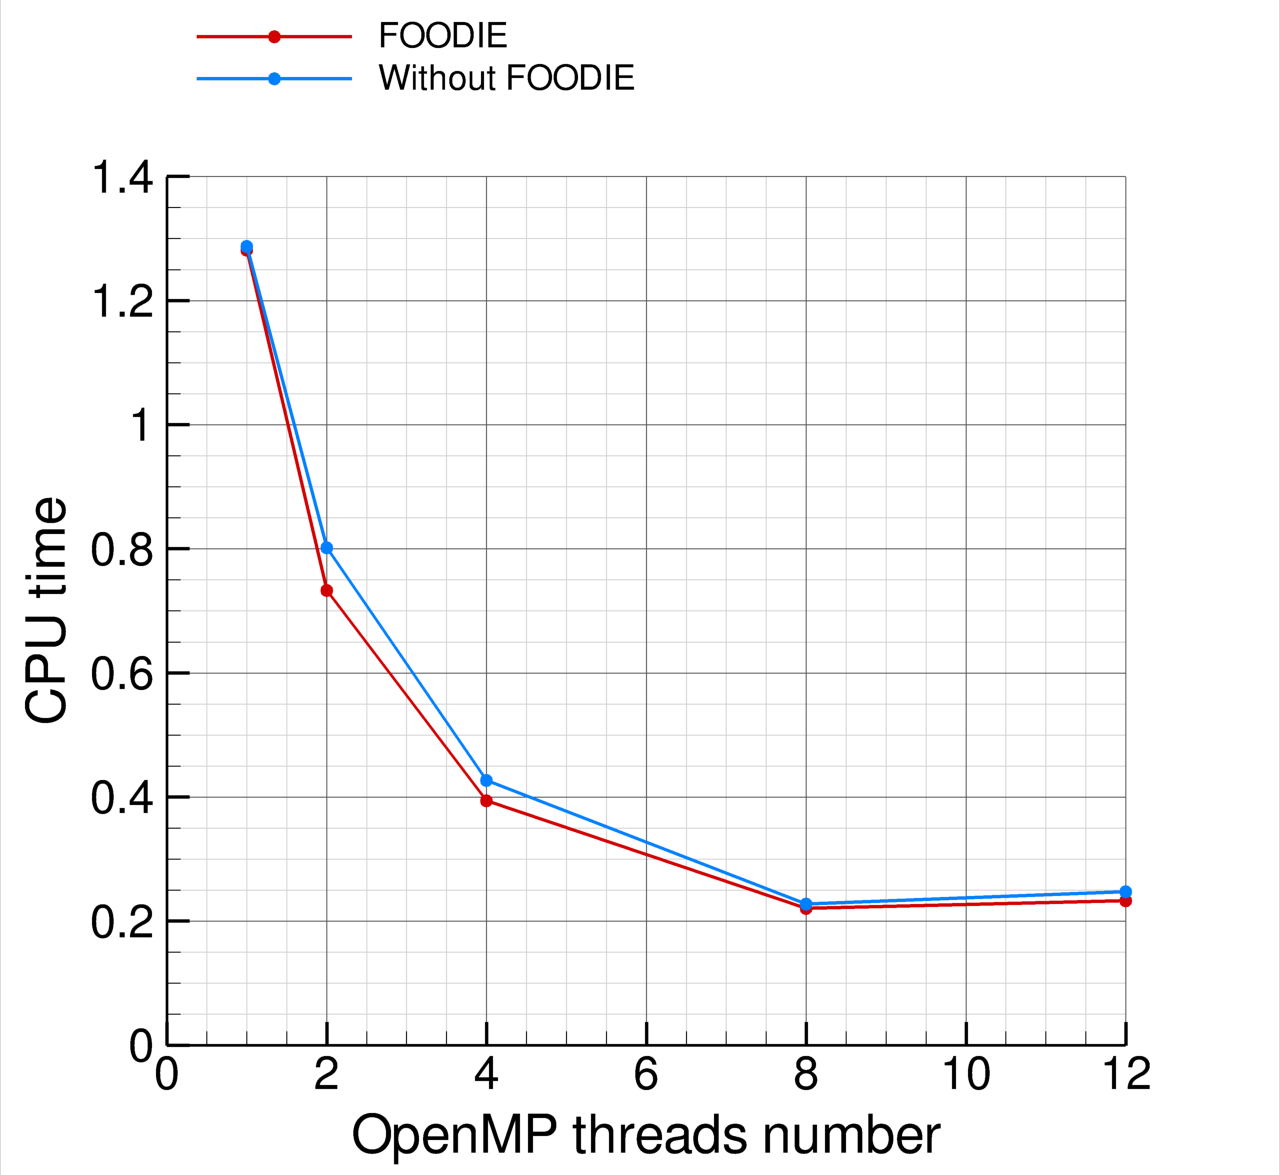
\includegraphics[width=1.00\textwidth]{openmp_benchmark/euler-1D-openmp/strong-cpu-time-comparison.png}
    \caption{Strong benchmark, number of cells 240000}\label{fig:strong-cpu-time-openmp}
  \end{subfigure}\quad%
  \begin{subfigure}[b]{0.40\textwidth}
    \centering
    \includegraphics[width=1.00\textwidth]{openmp_benchmark/euler-1D-openmp/weak-cpu-time-comparison.png}
    \caption{Weak benchmark, minimum number of cells 24000}\label{fig:weak-cpu-time-openmp}
  \end{subfigure}\\
  \caption{CPU time consumed with OpenMP programming model}\label{fig:cpu-time-openmp}
\end{figure}



\subsection{MPI benchmark}\label{subsec:mpi}

{\color{red} To be written.}
